\begin{minipage}{.3\textwidth}
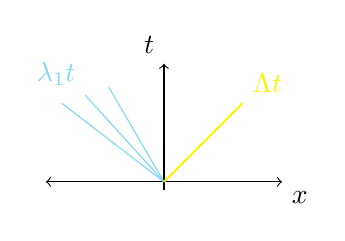
\begin{tikzpicture}
% coord.
\draw[<->] (-1.5,0) -- (1.5,0) node[anchor= north west] {$x$};
\draw[->] (0,-0.1) -- (0,1.5) node[anchor=south east] {$t$};
% contact disc
\draw[color=yellow, line width=0.25mm] (0,0) -- (1,1) node[anchor= south west] {$\Lambda t$};
% rarefaction
\draw[color=cyan!50!white] (0,0) -- (-1.3,1);
\draw[color=cyan!50!white] (0,0) -- (-1,1.1) node[anchor= south east] {$\lambda_1 t$};
\draw[color=cyan!50!white] (0,0) -- (-0.7,1.2);
%\node at (1.2,-0.5) {$(3a)$};
\end{tikzpicture}
%\caption{Slow rarefaction (blue) followed by a phase transition (yellow).}
%\label{Fig:SolRPRarefactionDiscCongestedPhase}
\end{minipage}
\quad 
\begin{minipage}{.3\textwidth}
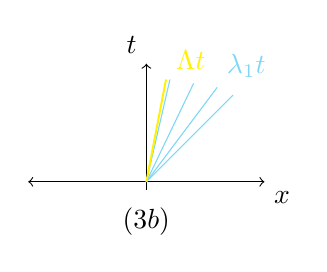
\begin{tikzpicture}
\draw[<->] (-1.5,0) -- (1.5,0) node[anchor= north west] {$x$};
\draw[->] (0,-0.1) -- (0,1.5) node[anchor=south east] {$t$};

\draw[color=cyan!50!white] (0,0) -- (1.1,1.1);
\draw[color=cyan!50!white] (0,0) -- (0.9,1.2) node[anchor= south west] {$\lambda_1 t$};
\draw[color=cyan!50!white] (0,0) -- (0.6,1.25);
\draw[color=cyan!50!white] (0,0) -- (0.3,1.3);
\draw[color=yellow, line width=0.25mm] (0,0) -- (0.25,1.3) node[anchor= south west] {$\Lambda t$};
\node at (0,-0.5) {$(3b)$};
\end{tikzpicture}
%\caption{Contact discontinuity followed by a contact discontinuity, $q_l = Q$.}
%\label{Fig: SolRPDiscCongestedPhase}
\end{minipage}
\quad 
\begin{minipage}{.3\textwidth}
\begin{tikzpicture}
\draw[<->] (-1.5,0) -- (1.5,0) node[anchor= north west] {$x$};
\draw[->] (0,-0.1) -- (0,1.5) node[anchor=south east] {$t$};
\draw[color=yellow, line width=0.25mm] (0,0) -- (1,1) node[anchor= south west] {$\Lambda t$};
%\draw[color=lime] (0,0) -- (-1,1) node[anchor= south east] {$\lambda_1 t$};
%\node at (1.2,-0.5) {$(3c)$};
\end{tikzpicture}
%\caption{A single phase transition (yellow) acting as a shock or contact.}
%\label{Fig: SolRPShockDiskCongestedPhase}
\end{minipage}

